\documentclass[10pt,twocolumn,letterpaper]{article}

\usepackage{cvpr}
\usepackage{times}
\usepackage{epsfig}
\usepackage{graphicx}
\usepackage{amsmath}
\usepackage{amssymb}
\usepackage{dsfont}
\usepackage{enumitem}
\usepackage{multicol}
\usepackage{multirow}
\usepackage{amsbsy}
\usepackage{array, floatrow, tabularx, makecell, booktabs}%

%%%%%%%%%%%%%%
% Packages and stuff custom
%%%%%%%%%%%%%%
\usepackage{url}
\usepackage{amsthm}
\usepackage{color}
\usepackage{subcaption}
\captionsetup{compatibility=false}
\usepackage{booktabs}
\usepackage{arydshln}
%\usepackage{hyperref}
% If you comment hyperref and then uncomment it, you should delete
% egpaper.aux before re-running latex.  (Or just hit 'q' on the first latex
% run, let it finish, and you should be clear).
\usepackage[pagebackref=true,breaklinks=true,letterpaper=true,colorlinks,bookmarks=false]{hyperref}

\DeclareMathOperator{\E}{\mathbb{E}}
\DeclareMathOperator{\R}{\mathbb{R}}

\def\figref#1{Fig.~\ref{#1}}
\def\secref#1{\S\ref{#1}}
\def\tabref#1{Table~\ref{#1}}
\def\eqnref#1{Eq.~\ref{#1}}

\newcommand{\ow}[1]{\textbf{\textcolor[rgb]{.1, .1, .8}{OW: #1}}}
\newcommand{\rz}[1]{\textbf{\textcolor[rgb]{.54, .16, .55}{RZ: #1}}}
\newcommand{\todo}[1]{\textbf{\textcolor[rgb]{.8, .1, .1}{#1}}}
\newcommand{\pd}[1]{\textbf{\textcolor[rgb]{1, 0.5, 0}{PD: #1}}}
\newcommand{\eli}[1]{\textbf{\textcolor[rgb]{0.1, 0.6, 0.1}{ES: #1}}}
\newcommand{\ag}[1]{\textbf{\textcolor[rgb]{0.45, 0.25, 0.1}{AG: #1}}}

%% spacehacks
%\setlength{\abovecaptionskip}{-5pt}


\newcommand{\addSubFigHalf}[3]{\begin{subfigure}[t]{.45\linewidth}
   \includegraphics[width=\linewidth]{#1}
   \caption{#2}\label{#3}\end{subfigure}
}
\newcommand{\addSubFigThird}[3]{\begin{subfigure}[t]{.31\linewidth}
   \includegraphics[width=\linewidth]{#1}
   \caption{#2}\label{#3}\end{subfigure}
}
\newcommand{\addSubFigTenth}[3]{\begin{subfigure}[t]{.16\linewidth}
   \includegraphics[width=\linewidth]{#1}
   \caption{#2}\label{#3}\end{subfigure}
}
\newcommand{\addSubFigSixth}[2]{\begin{subfigure}[t]{.12\linewidth}
   \includegraphics[width=\linewidth]{#1}
   \label{#2}\end{subfigure}
}
\newcommand{\addSubFigSixthLabel}[3]{\begin{subfigure}[t]{.12\linewidth}
   %\rotatebox{90}{#2}
   \includegraphics[width=.9\linewidth]{#1}
   \caption{#2}\label{#3}\end{subfigure}
}



\newcommand{\model}[0]{GateGAN}

\DeclareGraphicsExtensions{.pdf,.jpg}

%%%%%%%%%%%%%%%

\graphicspath{ {images/}{syntheticExp/} {final_images/channel_gated/} {final_images/} {paper_images/} }
%%%%%%%%%%%%%%%%


% Include other packages here, before hyperref.

% If you comment hyperref and then uncomment it, you should delete
% egpaper.aux before re-running latex.  (Or just hit 'q' on the first latex
% run, let it finish, and you should be clear).
\usepackage[pagebackref=true,breaklinks=true,letterpaper=true,colorlinks,bookmarks=false]{hyperref}

% \cvprfinalcopy % *** Uncomment this line for the final submission

\def\cvprPaperID{2914} % *** Enter the CVPR Paper ID here
\def\httilde{\mbox{\tt\raisebox{-.5ex}{\symbol{126}}}}

% Pages are numbered in submission mode, and unnumbered in camera-ready
\ifcvprfinal\pagestyle{empty}\fi
\begin{document}

%%%%%%%%% TITLE
\title{GAN-Gate: Conditional Gating for Image-to-Image Translation \\ Supplementary Material}
% \title{GAN-Gate: Gated Residual GANs for Class-Conditioned Image Generation}
% GAN-Gate: Conditionally-Gated Residual Networks for Image-to-Image Translation
% GAN-Gate: Softly-Gated Conditional Residual Networks for Image-to-Image Translation
% GAN-Gate: Conditionally Soft-Gated Residual Networks for Image-to-Image Translation
%GAN-Gate: Conditional Gating for Image-to-Image Translation

\author{Arnab Ghosh\\
University of Oxford\\
{\tt\small arnab.ghosh@eng.ox.ac.uk}
% For a paper whose authors are all at the same institution,
% omit the following lines up until the closing ``}''.
% Additional authors and addresses can be added with ``\and'',
% just like the second author.
% To save space, use either the email address or home page, not both
\and
Puneet Dokania\\
University of Oxford\\
{\tt\small puneet@robots.ox.ac.uk}
\and
Richard Zhang\\
Adobe Research\\
{\tt\small rizhang@adobe.com}
\and
Oliver Wang\\
Adobe Research\\
{\tt\small owang@adobe.com}
\and
Philip Torr\\
University of Oxford\\
{\tt\small philip.torr@eng.ox.ac.uk}
\and
Eli Shechtman\\
Adobe Research\\
{\tt\small elishe@adobe.com}
}

\maketitle

\begin{figure*}[t]
    \centering
    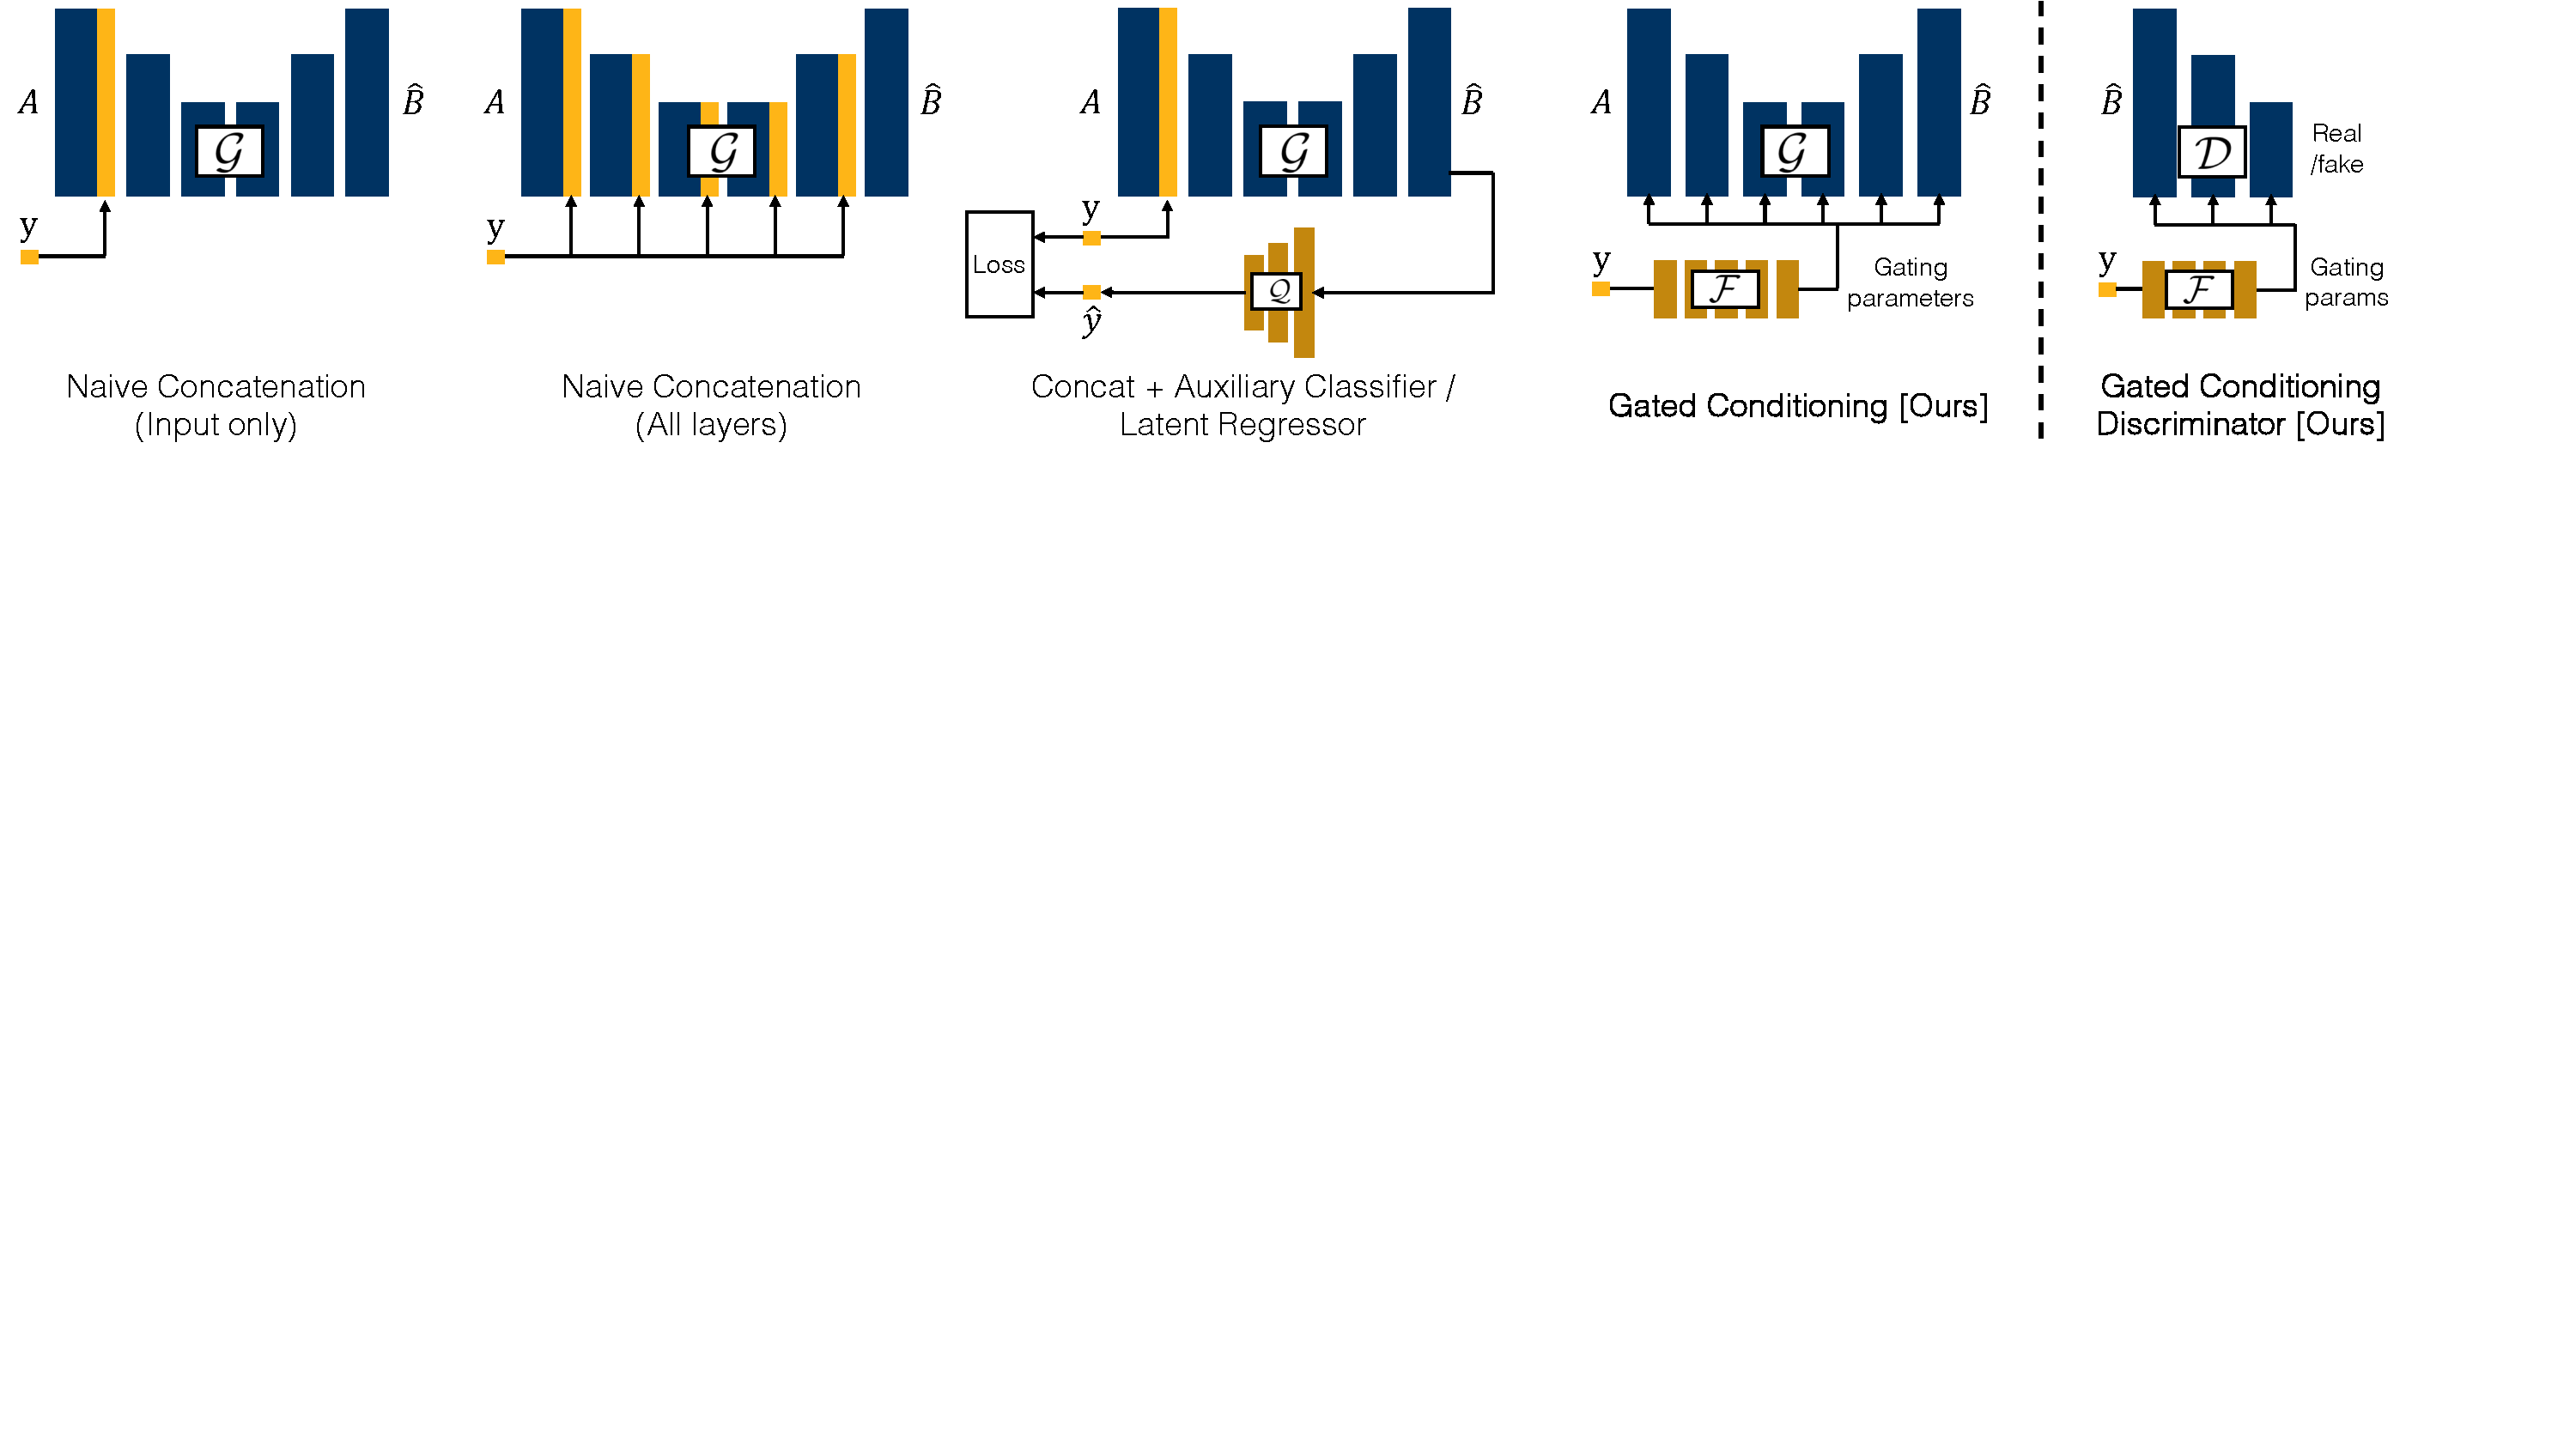
\includegraphics[width=\linewidth]{paper_images/arch_inject2.pdf}
    \caption{{\bf Conditioning injection variants.}
    The conditioner can be naively incorporated in a generator through simple concatenation in {\bf (left)} the input layer only or {\bf (mid-left)} in all layers. {\bf (mid)} The network can be further encouraged to use the conditioning through a learned network, using either a classification objective for categorical conditioning~\cite{odena2016conditional,chen2016infogan} or a regression objective for continuous conditioning. {\bf (Mid-right)} We train a network on the conditioner to predict parameters which guide softly-gated units in the main network. {\bf (Right)} These conditioning options can be correspondingly applied to a discriminator. We propose using soft-gating on the discriminator as well.\label{fig:arch-inj}
    \vspace{-2mm}
    }
    \vspace{-2mm}
\end{figure*}
\begin{figure*}[t]
\centering
\begin{tabular}{*{3}{c@{\hspace{3px}}}}
\textbf{Blockwise Gating} & \textbf{Channelwise Gating} \vspace{-1mm} & \\
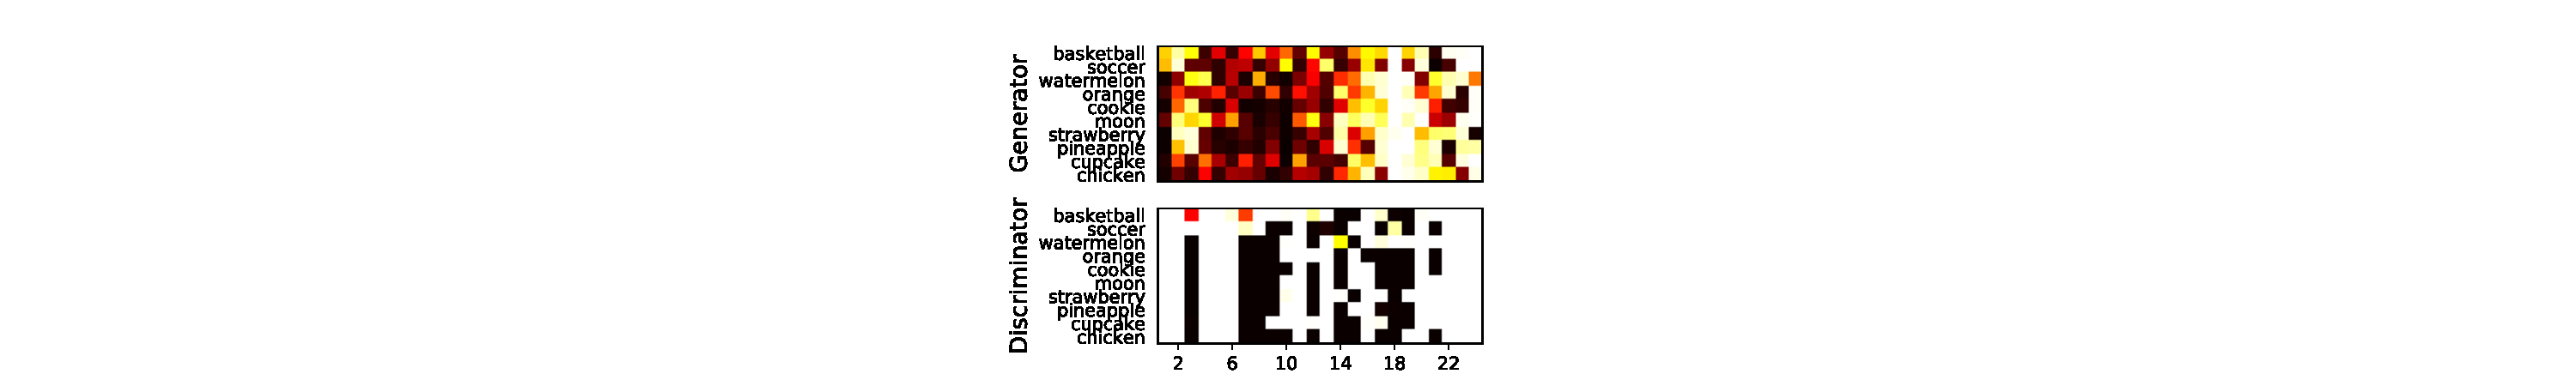
\includegraphics[height=3.35cm,trim={.15cm 0 0 .4cm}, clip]{paper_images/alphas_block.pdf} &
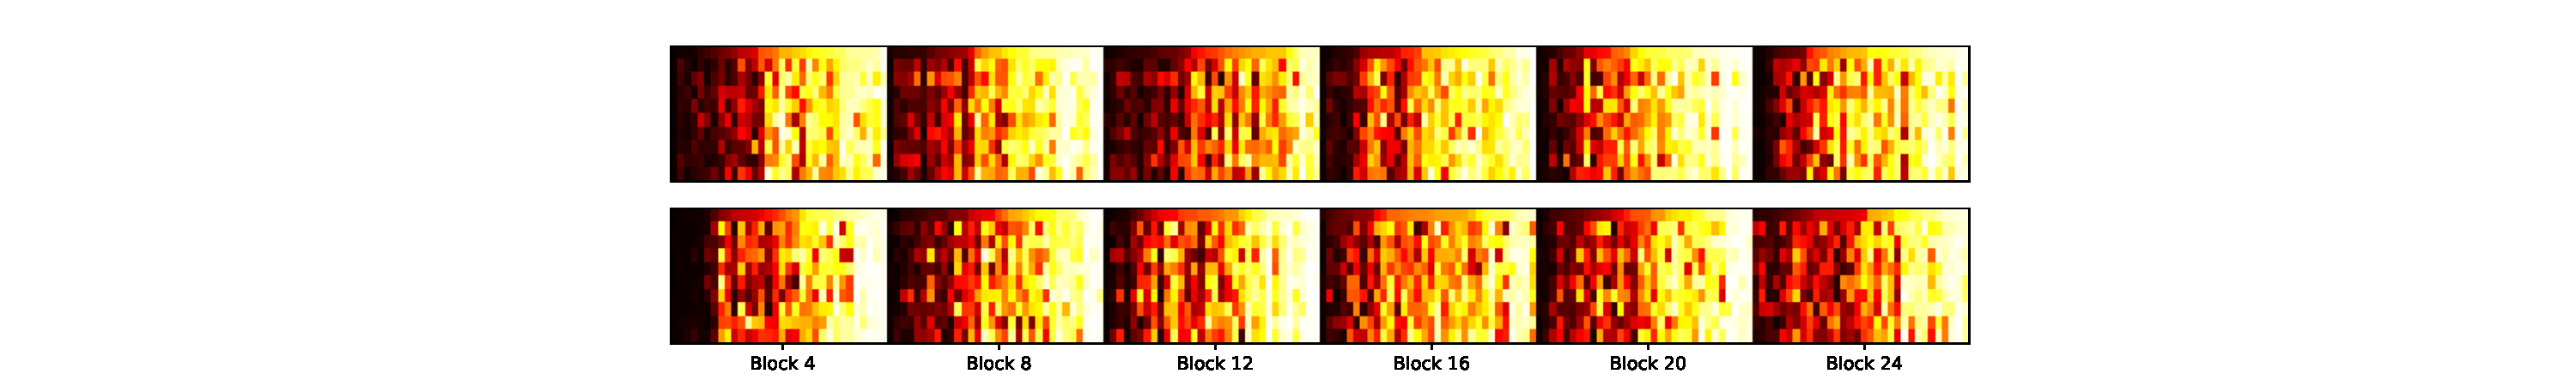
\includegraphics[height=3.35cm,trim={0 0 0 .4cm}, clip]{paper_images/alphas_chan.pdf} & 
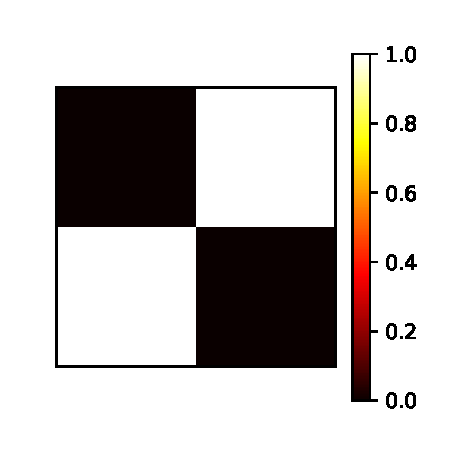
\includegraphics[height=3.35cm,trim={5.8cm 0 .2cm .4cm}, clip]{paper_images/alpha_legend.pdf}
\\
\end{tabular}
\vspace{-2mm}
\caption{\label{fig:alpha_heat}
\textbf{Learned gating parameters.} We show the soft-gating parameters for {\bf (left)} blockwise and {\bf (right)} channelwise gating for the {\bf (top)} generator and {\bf (bot)} discriminator. Black indicates
% $\alpha=0$, or
completely off, and white indicates
% $\alpha=1$, or 
completely on. For channelwise, a subset (every 4th) of blocks is shown. Within each block, channels are sorted in ascending order of the first category. The nonuniformity of each columns indicates that different channels are used more heavily for different classes.
\vspace{-3mm}
}
\vspace{-2mm}
\end{figure*}

\begin{figure*}[t]
    \centering
    % 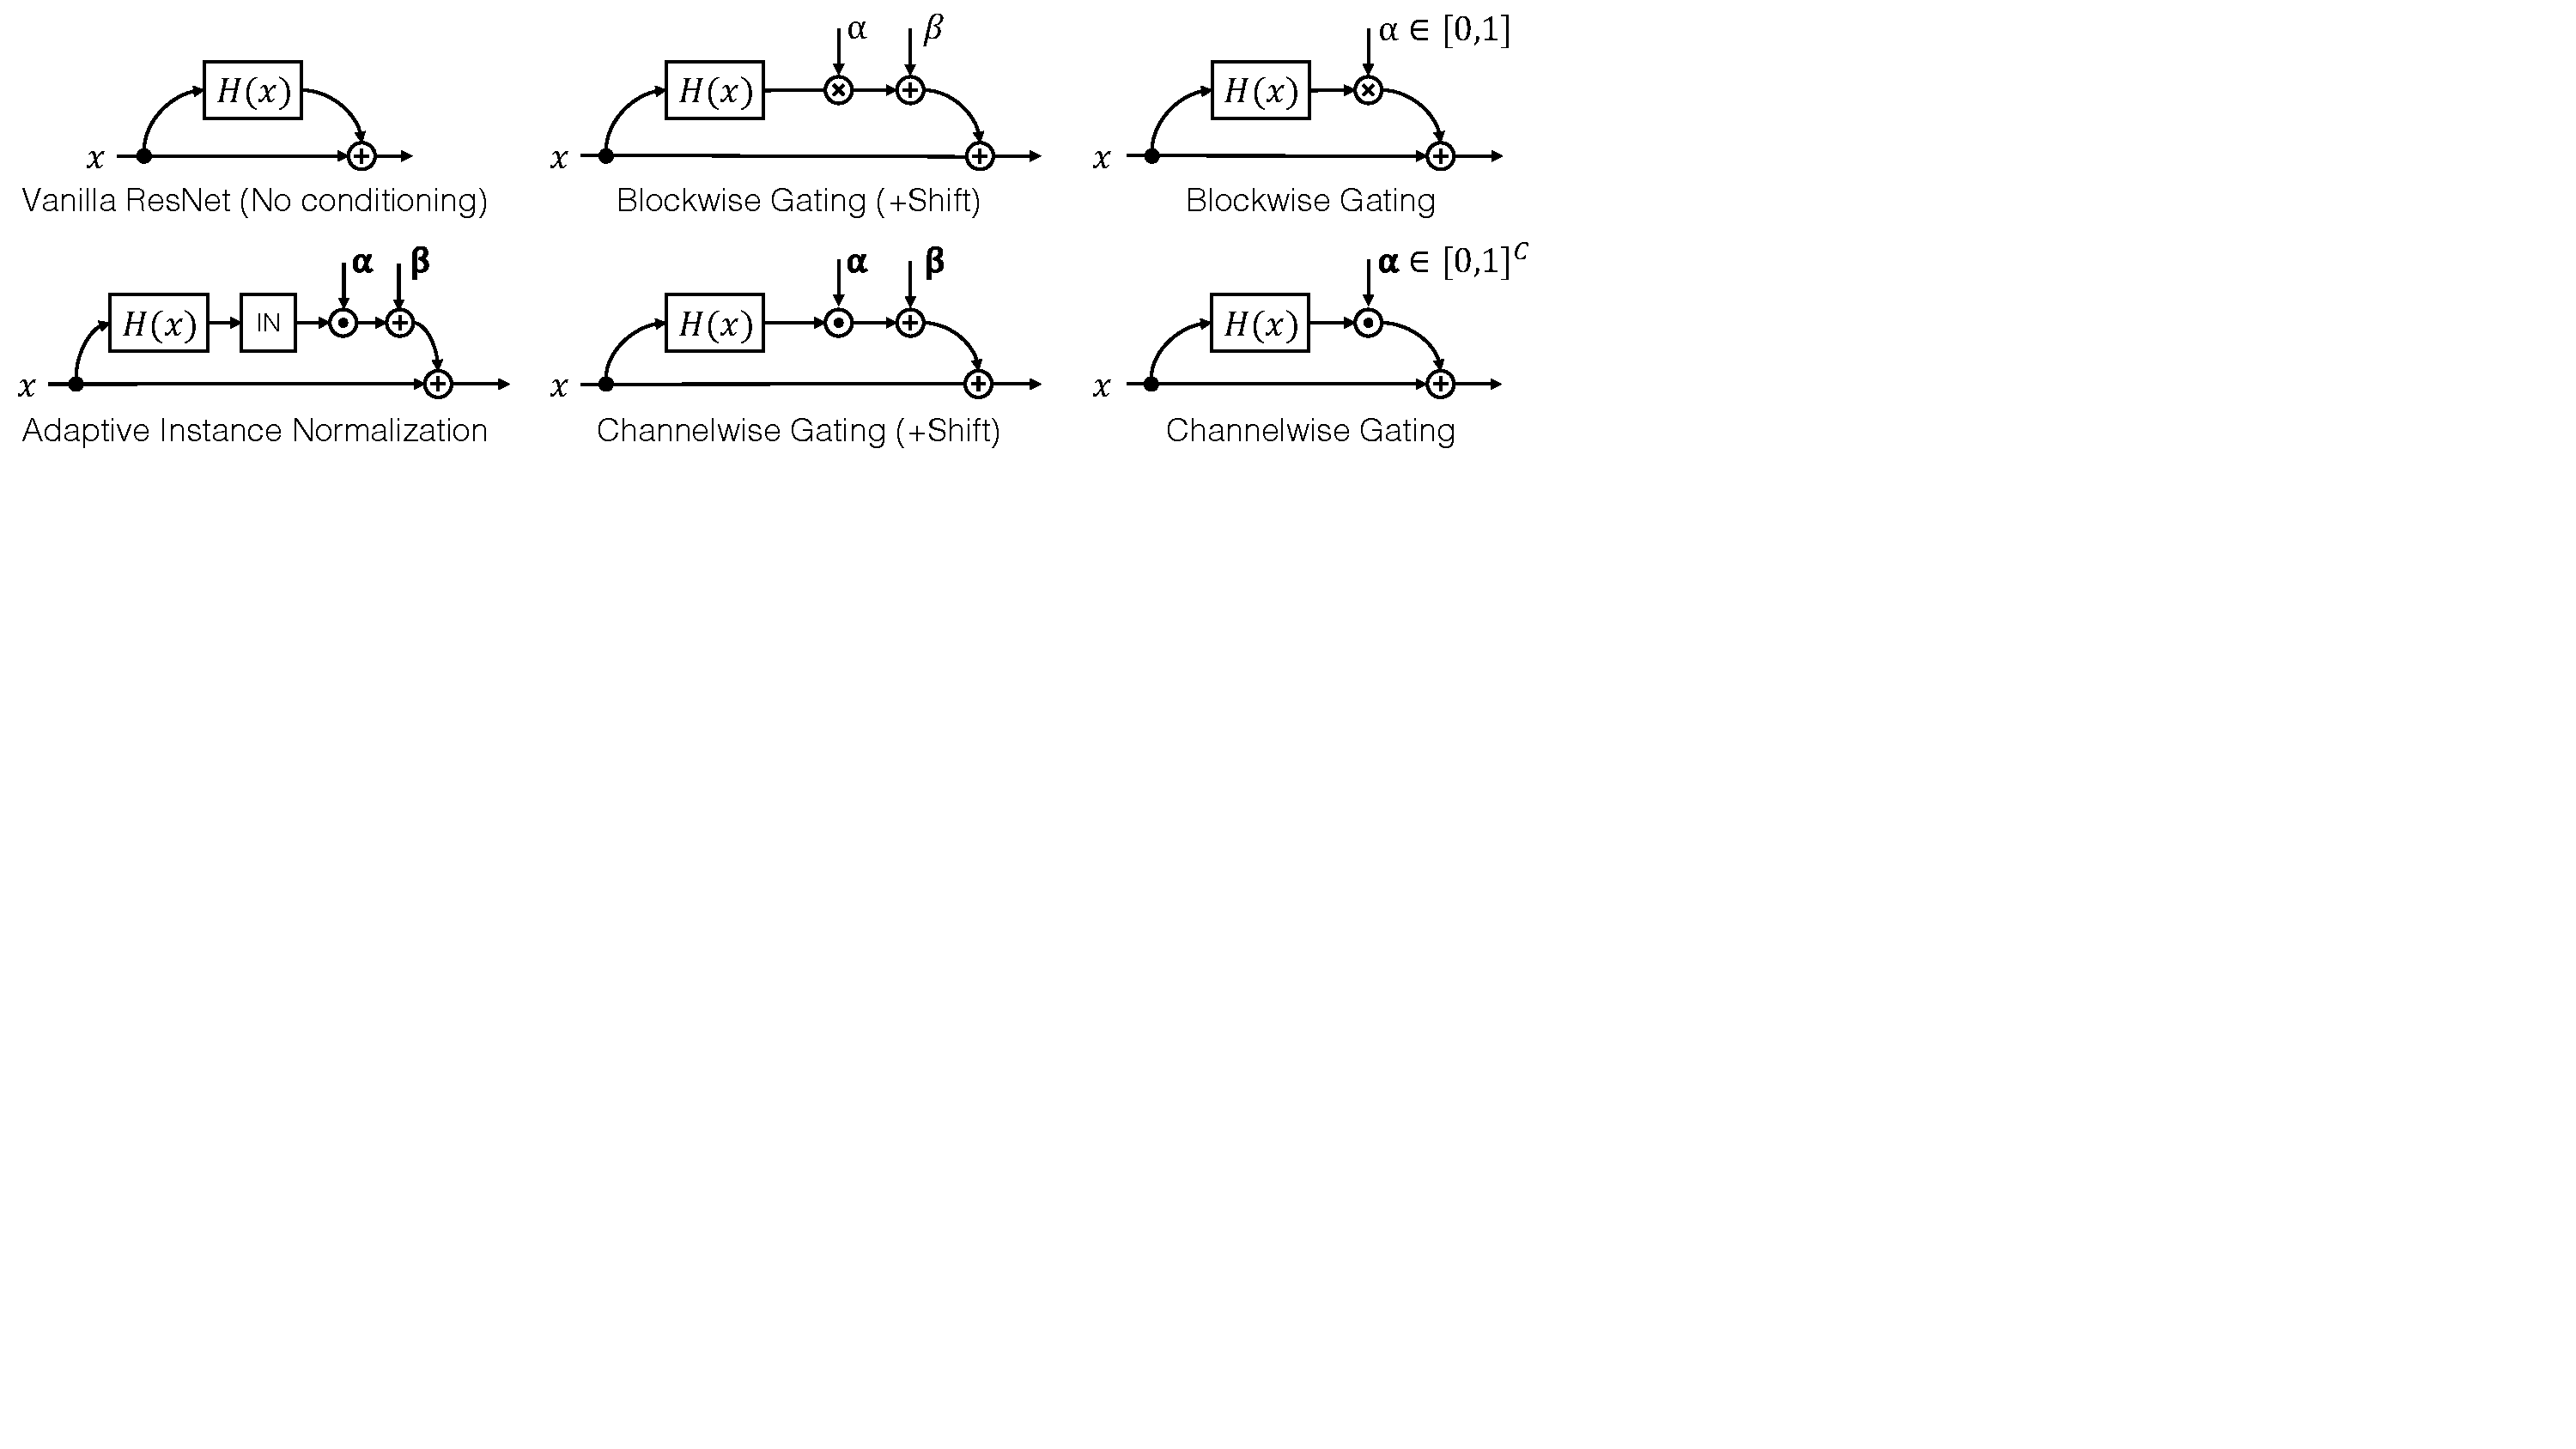
\includegraphics[width=\linewidth]{paper_images/arch_gate.pdf}
    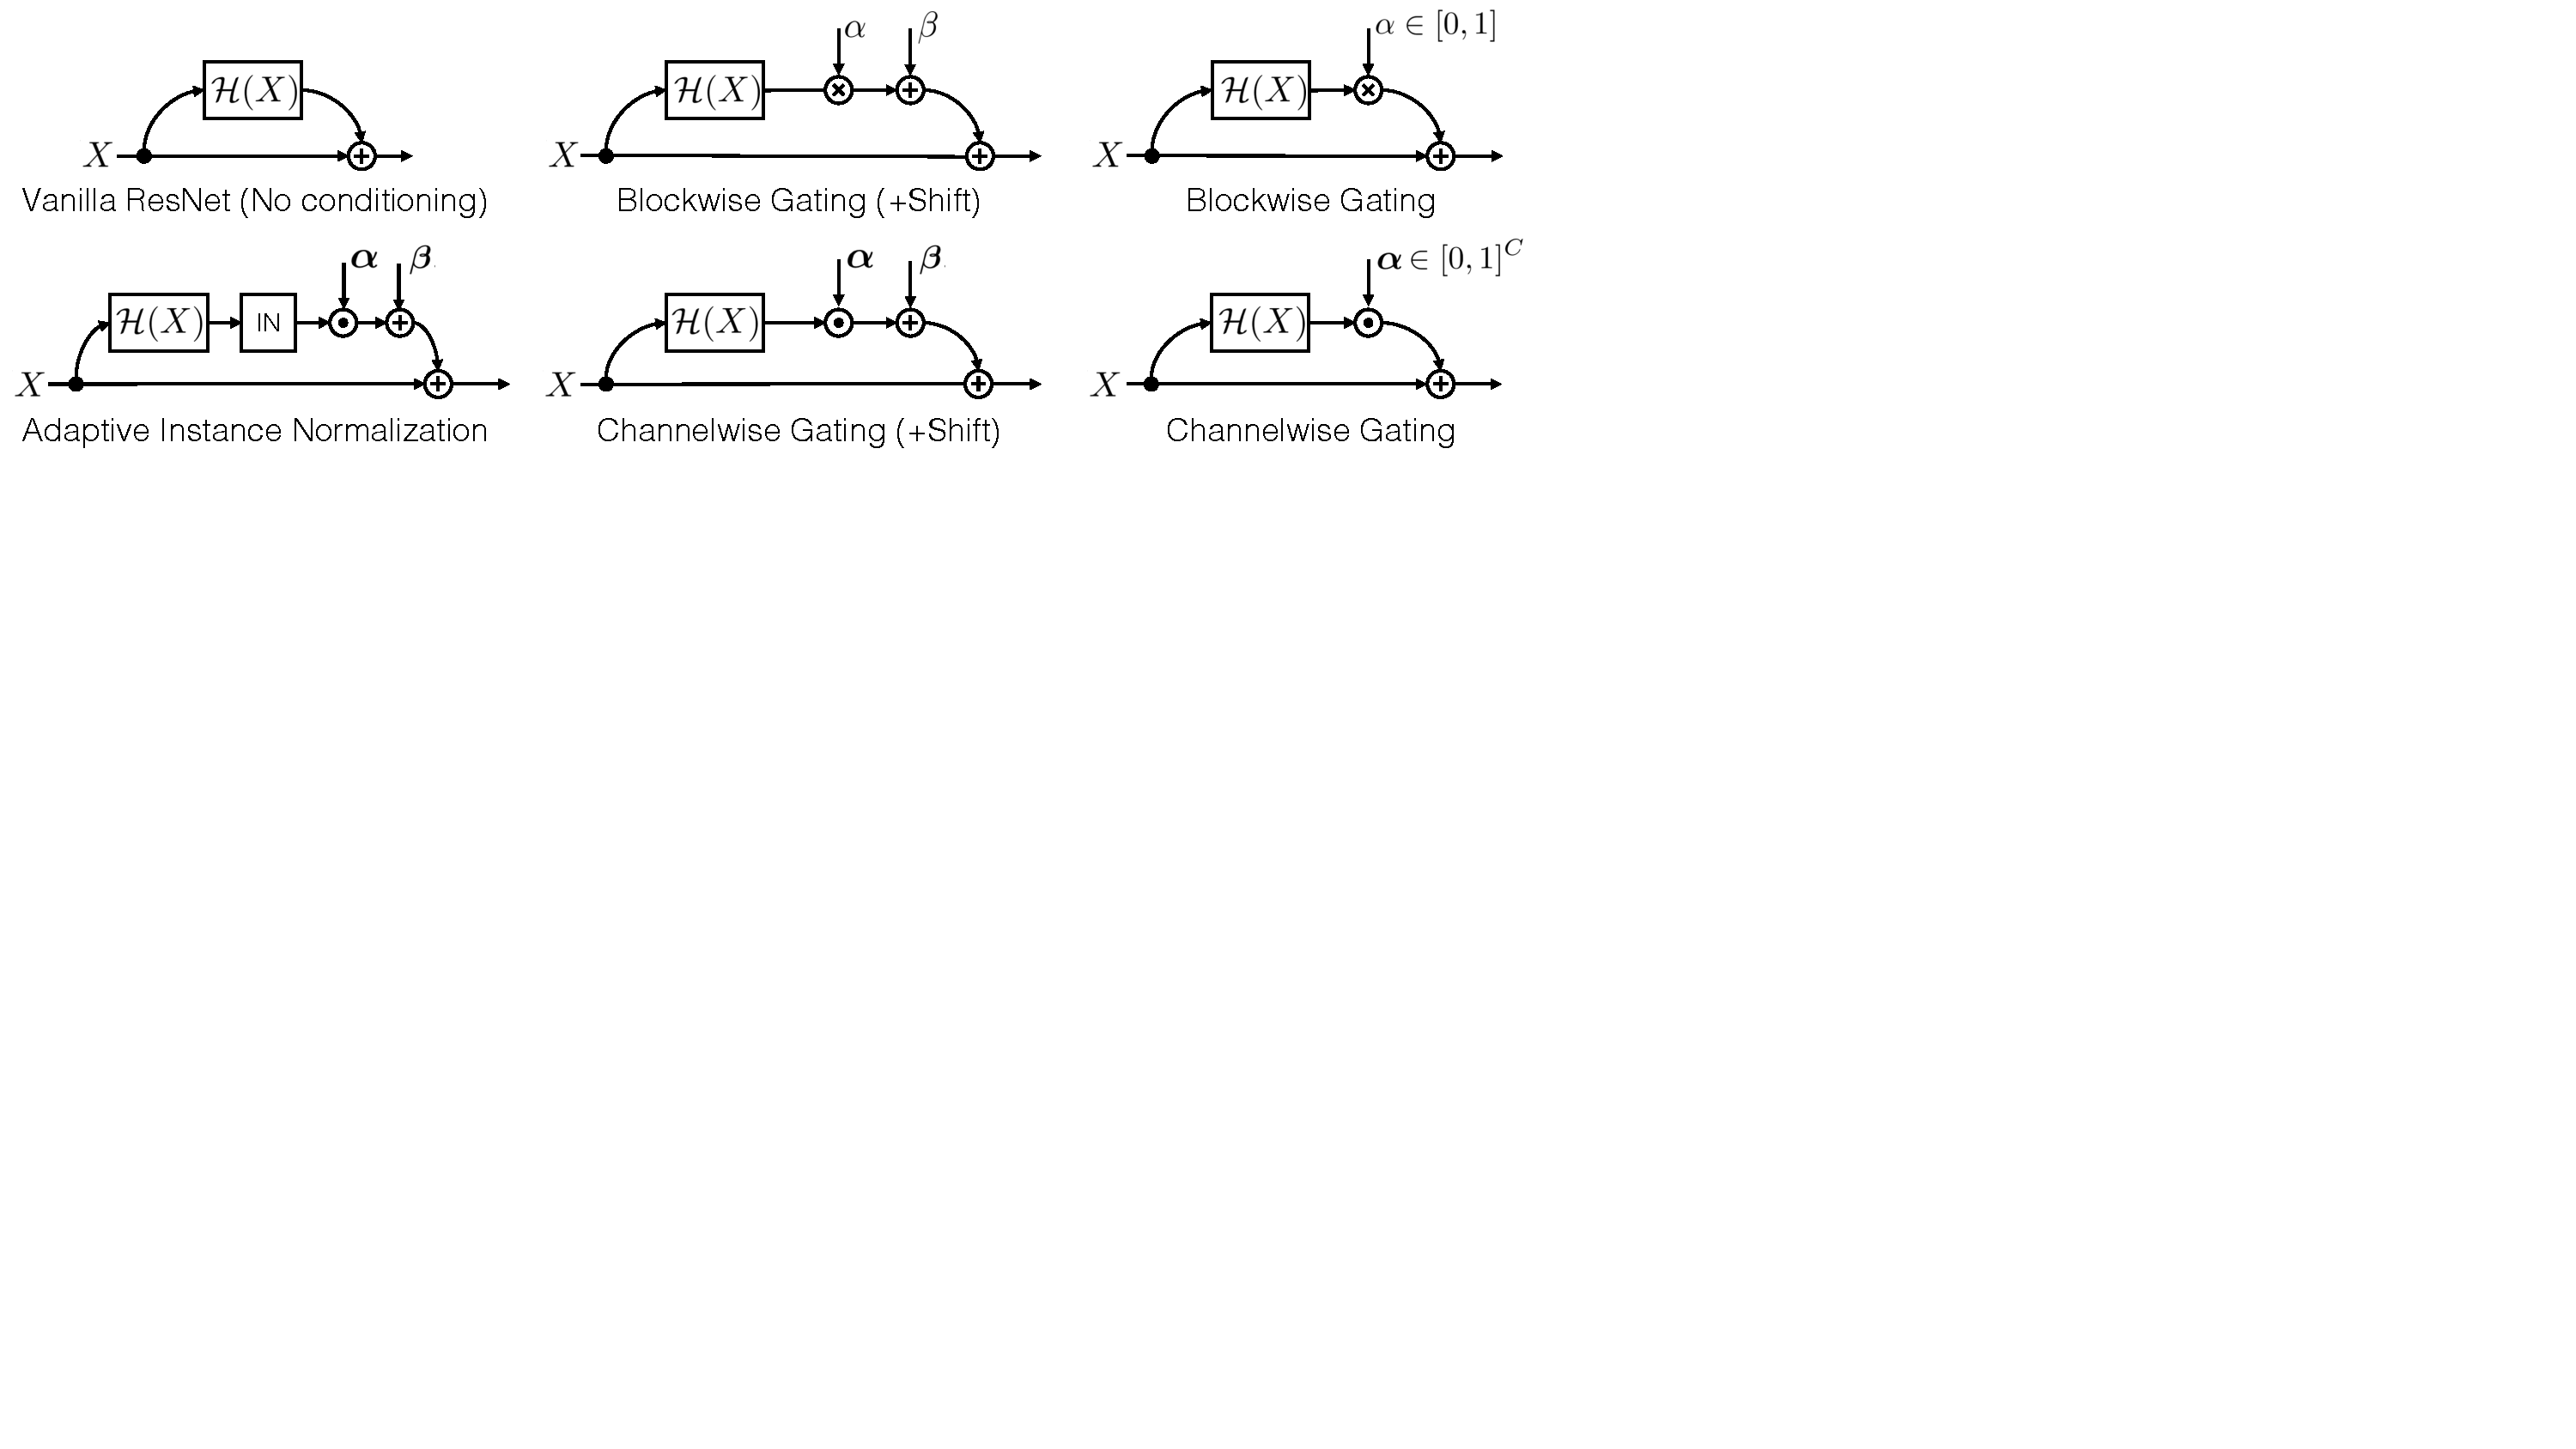
\includegraphics[width=.9\linewidth]{paper_images/arch_gate2.pdf}
    \caption{
    % {\bf Incorporating soft-gating into residual blocks.} \rz{Order got changed, may or may not need to add key for hadamard product}
    {\bf (Top-left)} A ``vanilla" residual block without gated conditioning parameters modifies input tensor $X$ into $X+\mathcal{H}(X)$. Conditioning with concatenation uses this setup. {\bf (Top-mid)} The $\mathcal{H}(X)$ block is softly-gated by scalar parameter $\alpha$ and shift $\beta$. {\bf (Top-right)} Only the gating is used, without bias. {\bf (Bot-left)} Adaptive Instance Normalization~\cite{huang2017arbitrary} applies a channel-wise scaling and shifting after an instance normalization layer. {\bf (Bot-mid)} Channel-wise gating adds restrictions to the range of $\mbox{\boldmath $\alpha$}$. {\bf (Bot-right)} We find that channel-wise gating (without added bias) to empirically produce the best results.\label{fig:arch-gate}
    \vspace{-2mm}
    }
    % \vspace{-4mm}
\end{figure*}

\begin{figure*}[h]
    \centering
    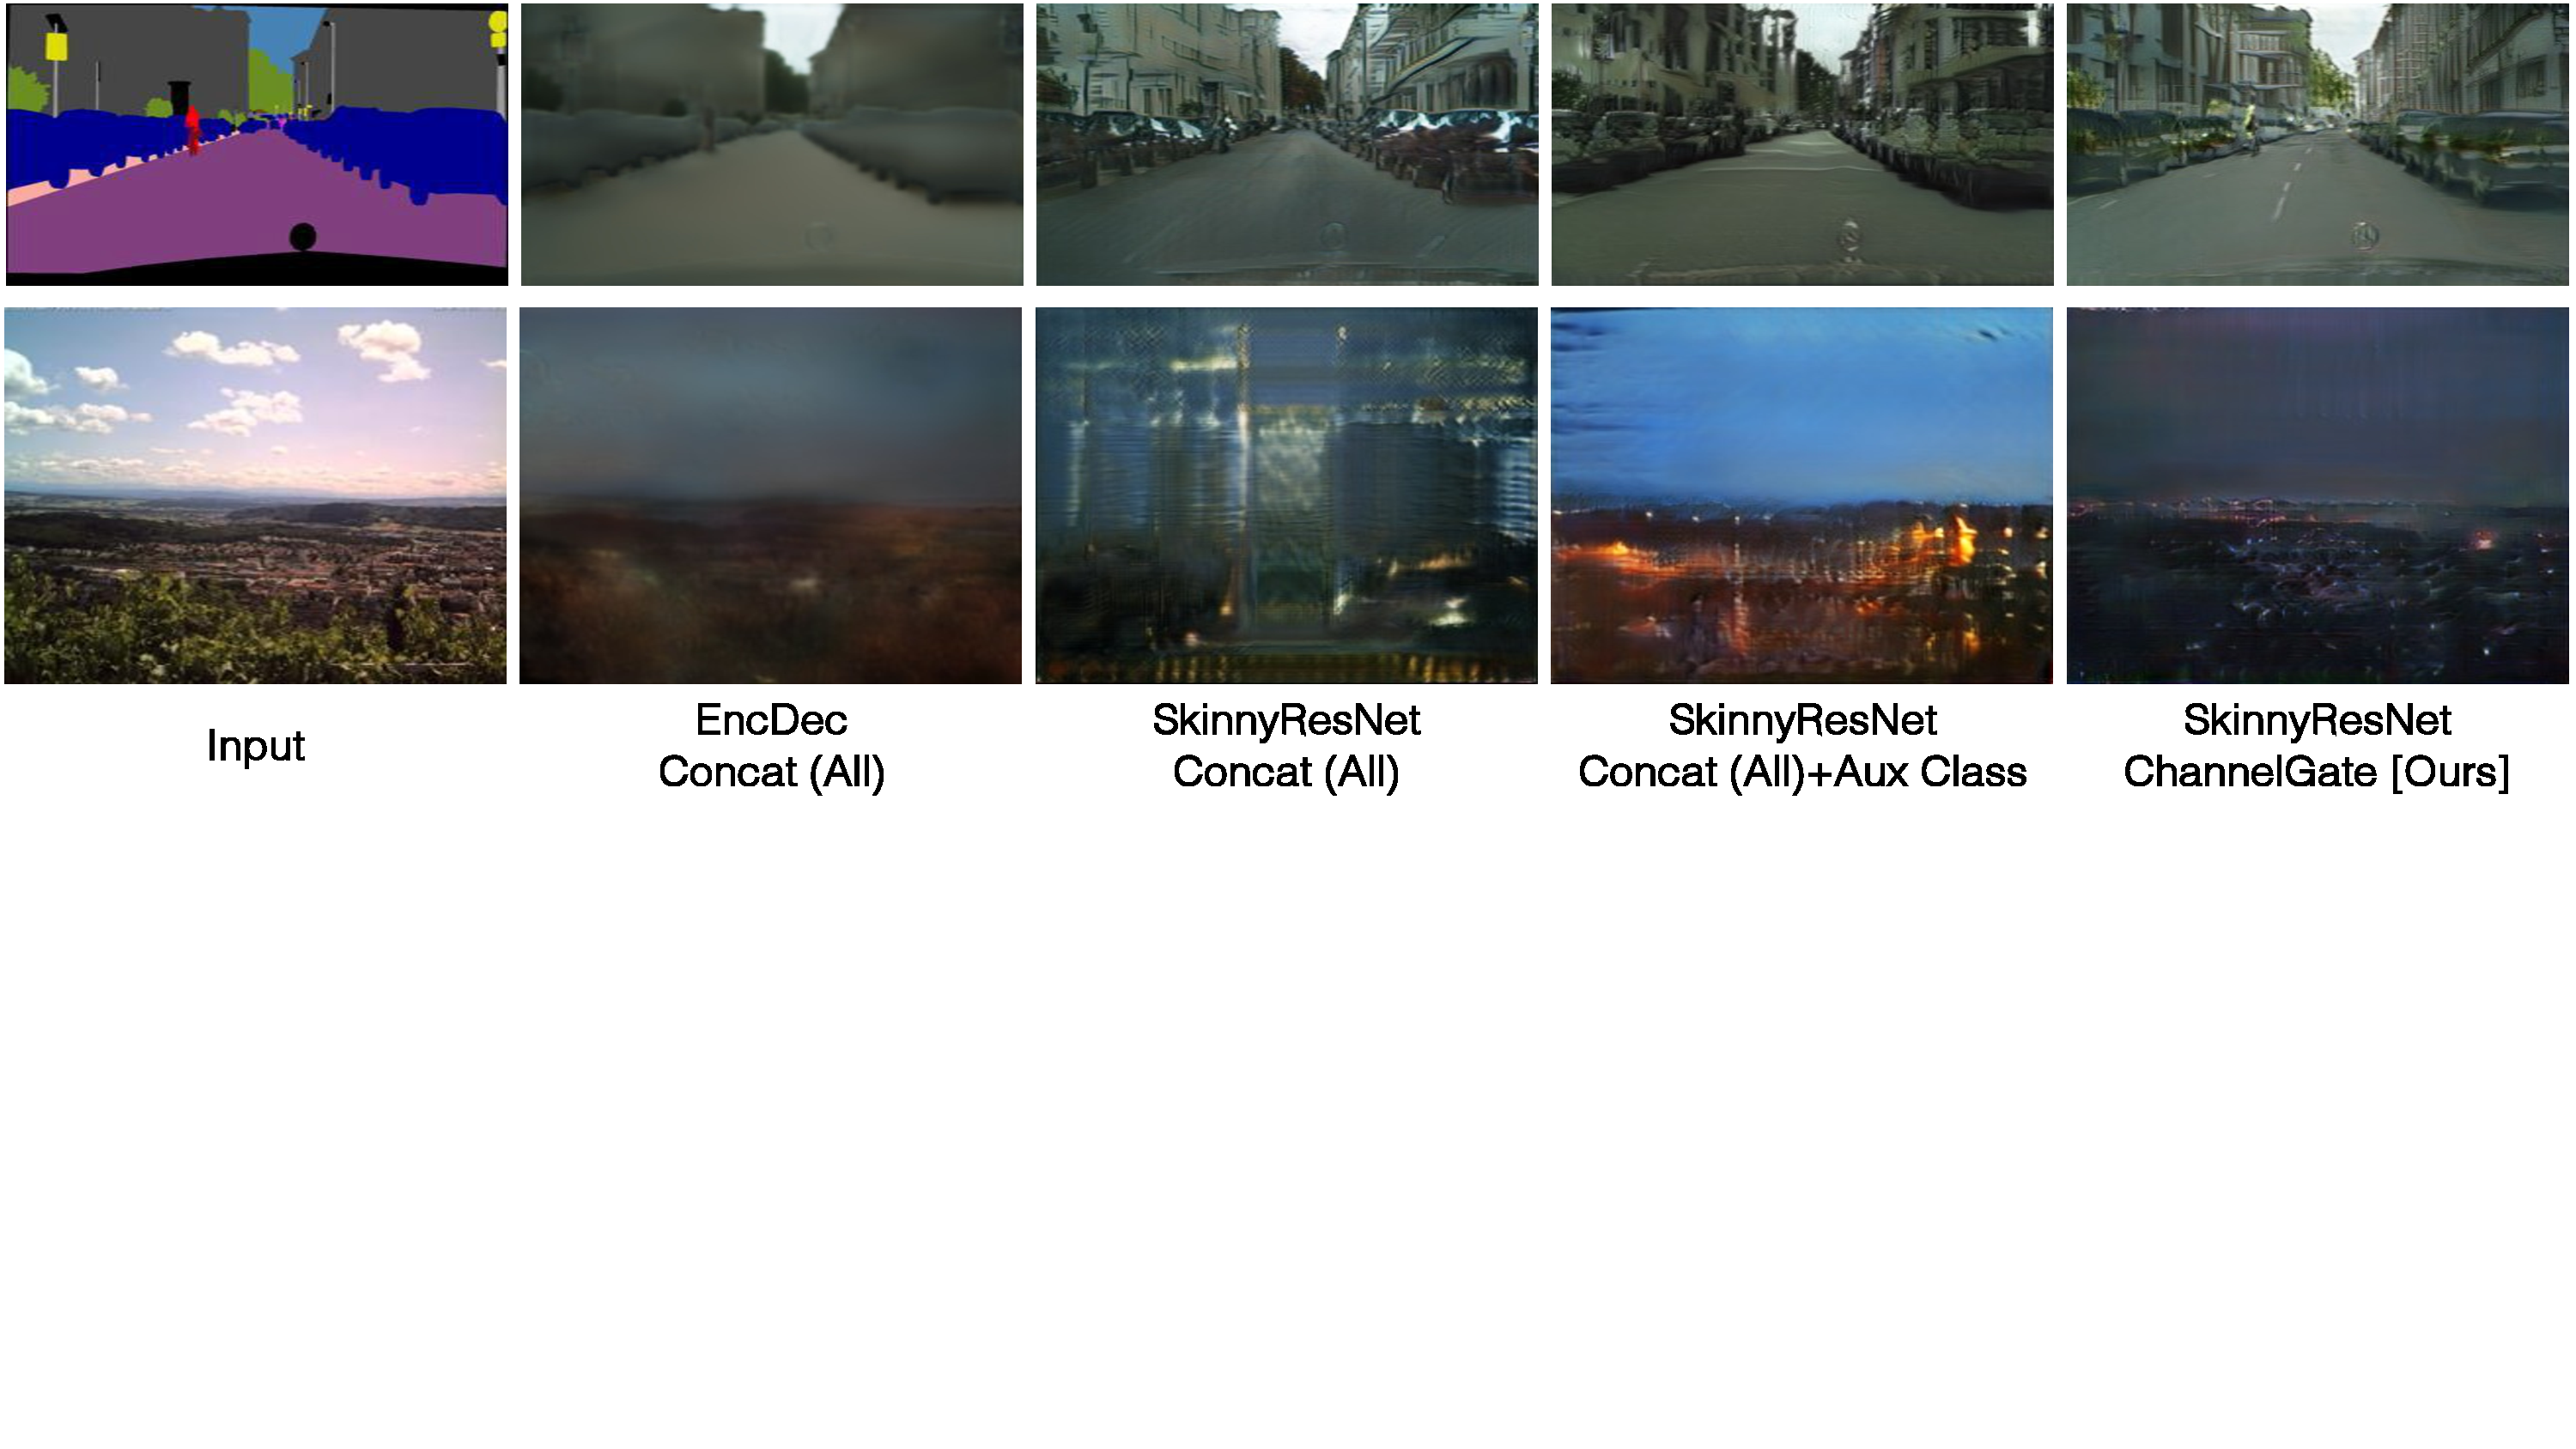
\includegraphics[width=1.\linewidth]{paper_images/multitask_comp.pdf}
    \caption{\textbf{Multitask generation results}. A single network trained on both Cityscapes Label$\rightarrow$Image and Day$\rightarrow$Night. The proposed channelwise gating method (right) is able to better incorporate task conditioning and produces more realistic results.
    % \ow{seems like this is missing 1. two generators, and 2. one generator. instead it seems more like an ablation study on our method, which is not the point. would be more impressive to show it matches 2 generators and 1 generator totally fails.}
    }
    \label{fig:multi-task_day2night}
    \vspace{-2mm}
\end{figure*}


\begin{table*}[t]
  \floatsetup{floatrowsep=qquad, captionskip=4pt}
  \centering
    \begin{floatrow}[2]
    \ffigbox[\FBwidth]{
    \scalebox{0.95} {
        \begin{tabular}{l c}
        % \hline
        \toprule
        \textbf{Model} & \textbf{LPIPS Distance} \\ \midrule
        Random Real Images & $0.3665 \pm 0.0053$ \\ \midrule
        BicycleGAN~\cite{zhu2017toward} & $0.1374 \pm 0.0005$  \\ \midrule
        Concat(In) &  $0.0432 \pm 0.0002$ \\
        Concat(All) & $0.0159 \pm 0.0004$ \\ \cdashline{1-2}
        ChannelGate [Ours] & $0.0964 \pm 0.0003$  \\
        \bottomrule %inserts single line
        \end{tabular}}}
        {\caption{\label{table:infogan_lpips} {\bf Edges$\rightarrow$Handbags Diversity.} LPIPSv0.1~\cite{zhang2018unreasonable} distance between randomly generated handbags, given the same edge map, as proposed in~\cite{zhu2016generative}. Given the same architecture, gating achieves higher diversity than concatenation.}}
        \ffigbox[\FBwidth]{
        \scalebox{0.95} {
        \begin{tabular}{l c c c} % 
        % \begin{tabular}{p{6cm}c{1.8cm}c{1.8cm}c{1.8cm}} % centered columns (4 columns)
        \toprule
        \multirow{2}{*}{\textbf{Model}} & \textbf{Per-pixel} &  \textbf{Per-class } & \textbf{Class} \\
        & \textbf{Acc} &  \textbf{Acc} & \textbf{IOU} \\ \midrule
        Pix2pix \cite{isola2016image2image} & 0.660  & 0.23 & 0.17 \\ \midrule
        EncDec, Concat(All) & 0.600 & 0.16 & 0.15 \\ \cdashline{1-4}
        SkinnyResNet, Cat(All) & 0.602 & 0.18 & 0.16 \\
        SkinnyResNet, Cat(All)+Aux-Class & 0.675 & 0.20 & 0.16 \\ \cdashline{1-4}
        SkinnyResNet, ChannelGate [Ours] & 0.684 & 0.23 & 0.18 \\ \bottomrule
        % \bottomrule %inserts single line
        \end{tabular}}}{
        \caption{ {\bf Cityscapes generation accuracy}. We evaluate the accuracy of Cityscapes Label$\rightarrow$Image generation results, as part of the multitask test. The network is also trained for an unrelated Day$\rightarrow$Night task. A pre-trained segmentation network, as used in~\cite{isola2016image2image} evaluates the synthesized results. Gating achieves higher results than concatenation, as well as single-task pix2pix~\cite{isola2016image2image}. }
        \label{label:me}}
    
    \vspace{-3mm}
  \end{floatrow}
%  \vspace{-2mm}
%   \label{fig:real_vs_div}
\end{table*}

\vspace{-1mm}
\subsection{Multi-Task Generation}
We also evaluate two previously shown image-to-image translation tasks -- segmentation$\rightarrow$street scene, and day $\rightarrow$ night -- using the {\em same} network. 
%Since our network is robust enough to be able to generate images conditioned on class and modulation of which blocks to use, it can further be used to generate images which are different in tasks such as the same network
As shown in \figref{fig:multi-task_day2night}, our model (ChannelGate) is able to perform both tasks, while the the baselines generate mixed results. 

In the case of an \textbf{EncoderDecoder} architecture \cite{huang2018multimodal} conditioned using concatenation on all layers, the discriminator becomes too powerful, and the training progressed with only the L1 loss, resulting in blurry outputs. The other baselines based on our \textbf{SkinnyResNet} architecture failed to generate realistic images in the case of the task of day$\rightarrow$night, while our method can achieve both.



\end{document}